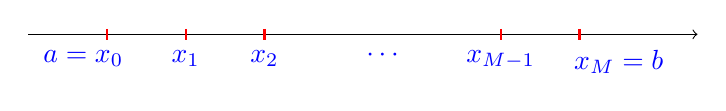
\begin{tikzpicture}
	\draw[->] (-1,0) -- (7.5,0);
		
	\foreach \i in {1,2}	
		\draw[red,thick] (\i,2pt)--(\i,-2pt) 
			node[text=blue,anchor=north]{$x_{\i}$};
	
	\draw[red,thick] (5,2pt)--(5,-2pt) 
		node[text=blue,anchor=north]{$x_{M-1}$};	
	\draw[red,thick] (0,2pt)--(0,-2pt)
		node[text=blue,anchor=north] at (-0.3,-2pt){$a=x_0$};
	\draw[red,thick] (6,2pt)--(6,-2pt) 
		node[text=blue,anchor=north] at (6.5,-2pt){$x_M=b$};
	\node[text=blue,anchor=north] at (3.5,-2pt) {$\cdots$};	
\end{tikzpicture}